% $Id: introduction.tex 87303 2016-02-08 13:44:29Z lafferty $
\subsection{Expected sensitivity}
\label{subsec:sensitivity}

The expected statistical precision on \BRof\Kspizmm for multiple values of the integrated luminosity up to 100 \invfb is estimated in this section.
% The fit to the available data performed in \secref{sec:fit} allows obtaining the model parameters of the background. 
The TIS samples used are equivalent to a 100\% trigger efficiency sample with an integrated luminosity of 4.9 and 0.77 \invpb for the FULL  and PARTIAL samples, respectively. %This effective luminosity, $L_{eff}^{dat}$, 
%has been estimated using the \Kspipi decays present in the sample, as well as the \Kspipi TIS efficiency, which is $\approx2\times10^{-3}$ as measured using the TISTOS method~\cite{TISTOS}.
The expected background yield is extrapolated from the current data fit result, where the signal yield is consitent with zero.
The background yield is scaled linearly for larger integrated luminosities.
%\begin{equation}
%N_{bkg}^L = N_{bkg}^{dat}\times\frac{L}{L_{eff}^{dat}}.
%\end{equation}

For each integrated luminosity in the studied range, sets of pseudo-experiments are generated  with the above background expectations,
and with a signal yield expectation of
\begin{equation} 
N_{sig} = \frac{\BRof\Kspizmm}{\BRof\Kspipi} \frac{\epsilon_{\KsPzMuMu}}{\epsilon_{\PKzS\to\Pgpp\Pgpm}}  N(\Kspipi)\times \frac{L_{fut}}{L_{curr}},
\end{equation} %dropped NA48 subindex for BR
% % where $\epsilon$ is the corresponding detection efficiency and 
where $L_{fut}$ and $L_{curr}$ are the future and current luminosities, respectively.
The models described in \secref{subsec:fit} are fit to each pseudo-experiment with a floating \BRof\Kspizmm.
The background model parameters used are the ones obtained from the fit to the data \secref{subsec:fit}. The statistical uncertainties
are obtained as the variations of \BRof\Kspizmm that deviate from the minimum of the log-likelihood profile by half a unit.
Finally, the uncertainties are averaged across the set of pseudo-experiments for a given integrated luminosity.
The uncertainties on the background extrapolation are large and translate into large uncertainties on the luminosity needed for achieving a given sensitivity. The resulting sensitivity curves are shown
in \figref{fig:sensitivity}.
It can be seen that the analyses of both PARTIAL and FULL categories can lead to a precision
better than NA48 for the LHCb upgrade if a trigger efficiency above $\approx 50\%$ can be maintained. The \KS production cross-section increases by $\approx20\%$ at 14 $\rm TeV$ compared to 8 $\rm TeV$, but this increase is cancelled by a 
larger fraction of \KS decaying outside of the VELO volume. For this reason, no energy correction has been applied to the sensitivity estimate.
Studies of \Kspizmm and minimum bias samples simulated with the LHCb upgrade detector and conditions show that the High Level
Trigger rate can be kept low enough for a 100 \% efficiency. Further timing studies are currently ongoing.


\begin{figure} [htb!]
\begin{center}
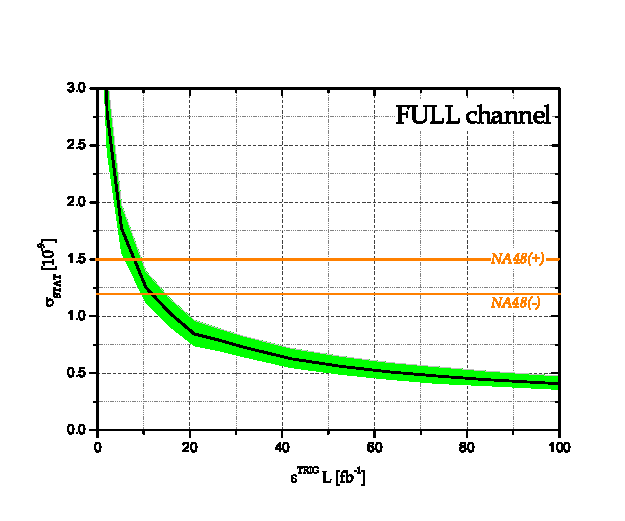
\includegraphics[scale=0.80]{figs/Kspi0MuMu/sensit_FULL.pdf}%{figs/sensitivity_more_colorfull.pdf}
\includegraphics[scale=0.80]{figs/Kspi0MuMu/sensitPARTIAL.pdf}
%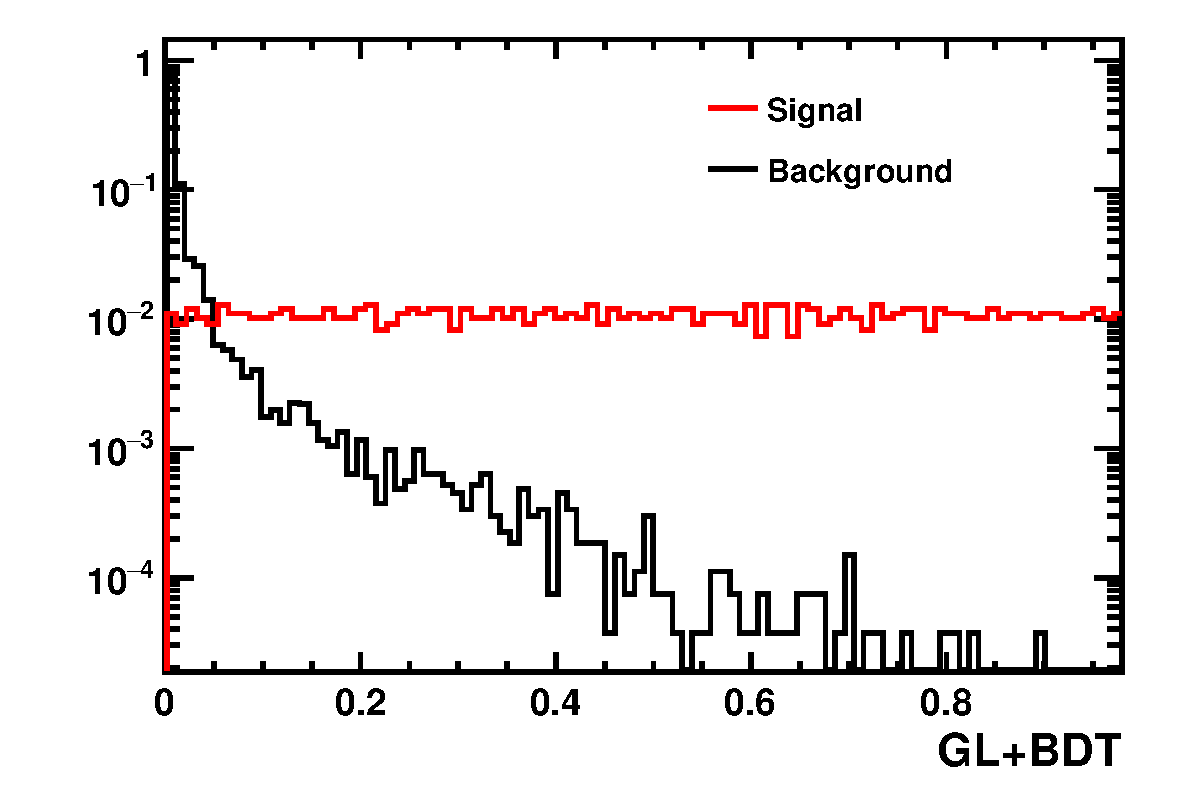
\includegraphics[scale=0.30]{figs/bdt_partial.pdf}
\caption{Expected precision on \BRof\Kspizmm for the FULL (top) and PARTIAL (bottom) channels, as a function of the integrated luminosity times trigger efficiency, $L\times\varepsilon^{TRIG/SEL}$. \label{fig:sensitivity}}
%The green line indicates the behavior of the precision extrapolating from the best fit value of the expected background. In the case of the black curve, this extrapolation is done averaging the background predictions within their uncertainties, while in the orange case the extrapolation takes as reference the best fit value of the expected background deviated one sigma from its mean value. \label{fig:sensitivity}}
\end{center}
\end{figure}


%\begin{figure} [htb!]
%\begin{center}
%\includegraphics[scale=0.60]{figs/sensitPARTIAL.pdf}
%%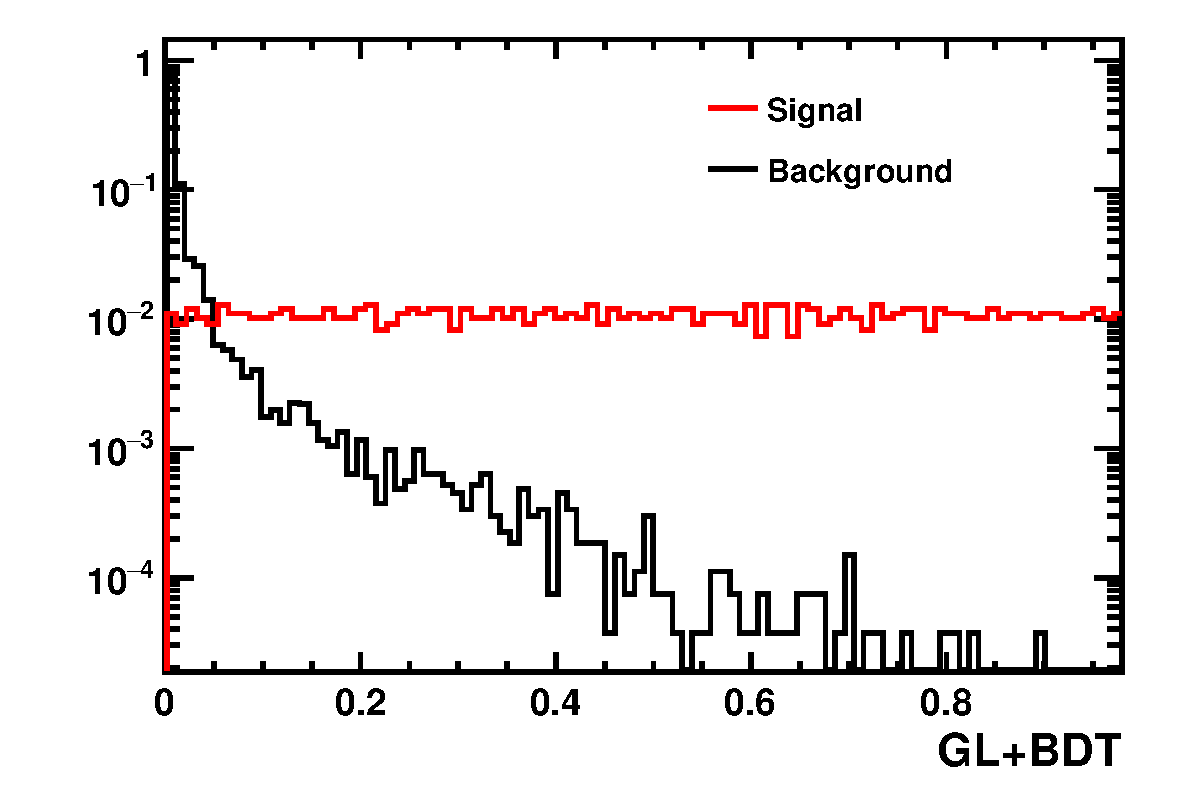
\includegraphics[scale=0.30]{figs/bdt_partial.pdf}
%\caption{Expected precision on \BRof\Kspizmm for the PARTIAL channel, as a function of the integrated luminosity times trigger efficiency, $L\times\varepsilon^{TRIG/SEL}$. The green 
%line indicates the behavior of the precision extrapolating from the best fit value of the expected background. In the case of the black curve, this extrapolation is done averaging the background 
%predictions within their uncertainties, while in the orange case the extrapolation takes as reference the best fit value of the expected background deviated one sigma from its mean value. {\it some lines are actually not there , but the plot in general needs to
%be updated} \label{fig:sensitivityPARTIAL}}
%\end{center}
%\end{figure}





 

